% =====================================================================
%  Makerere University MSc research proposal template
%  https://github.com/<your-username>/makerere-msc-proposal-template
%
%  Compile with pdfLaTeX; the bibliography runs through Biber.
%  On Overleaf: Menu -> Compiler = pdfLaTeX, Main document = main.tex.
%  Locally:     latexmk -pdf main.tex
%
%  Order of work:
%    1. metadata.tex   your name, title, supervisors, dates
%    2. frontmatter/   declaration, acknowledgements, abbreviations, summary
%    3. chapters/      your three chapters
%    4. backmatter/    budget and work plan
%    5. references.bib your references
%  preamble.tex holds the formatting and rarely needs editing.
% =====================================================================
\documentclass[12pt,a4paper,oneside]{report}

% =====================================================================
%  metadata.tex  --  EDIT THIS FILE FIRST
%  Everything specific to you and your proposal lives here. The title
%  page, the declaration and the PDF properties all read from it.
% =====================================================================

% ---- The proposal ---------------------------------------------------
\newcommand{\thesistitle}{Title of Your Research Proposal in Sentence or Title Case}
% Optional second line of the title. Leave empty if the title fits on one line.
\newcommand{\thesissubtitle}{}

% ---- The candidate --------------------------------------------------
\newcommand{\candidatename}{FIRSTNAME SURNAME}
\newcommand{\candidatepostnominal}{(BSc)}      % e.g. (BSc), (MSBS)
\newcommand{\registrationnumber}{20XX/HDXX/XXXXXU}

% ---- The degree -----------------------------------------------------
\newcommand{\degreename}{MASTER OF SCIENCE IN \MakeUppercase{your programme}}
\newcommand{\universityname}{MAKERERE UNIVERSITY}
\newcommand{\submissiondate}{Month DD, YYYY}

% ---- Supervisors ----------------------------------------------------
% Add or remove blocks in frontmatter/declaration.tex to match the
% number of supervisors. These commands hold the details of each.
\newcommand{\supervisorone}{%
  Supervisor One Name, PhD\\
  Title, Department,\\
  School, College,\\
  Makerere University,\\
  P.O. Box 7062, Kampala, Uganda.}

\newcommand{\supervisortwo}{%
  Supervisor Two Name, PhD\\
  Title, Institute or Programme,\\
  Organisation,\\
  P.O. Box XXXX, Kampala, Uganda.}

% ---- Logo -----------------------------------------------------------
% Replace figures/university_logo.png with your own institution's logo
% if you are not at Makerere. See the note in README.md.
\newcommand{\universitylogo}{figures/university_logo.png}

% =====================================================================
%  preamble.tex
%  All formatting for the Makerere University MSc proposal template.
%
%  A4, Times 12 pt, 1.5 line spacing, numbered hierarchical headings,
%  Roman pagination for the preliminary pages and Arabic for the main
%  text, table captions above and figure captions below, APA 7th edition
%  referencing through biblatex-apa and Biber.
%
%  Compiler: pdfLaTeX      Bibliography: Biber
%  You should not need to edit this file. Put your details in
%  metadata.tex and your text in chapters/.
% =====================================================================

\PassOptionsToPackage{hyphens}{url}

% ---- Page geometry -------------------------------------------------
\usepackage[a4paper,top=2.54cm,bottom=2.54cm,left=2.54cm,right=2.54cm]{geometry}

% ---- Fonts and encoding --------------------------------------------
\usepackage[T1]{fontenc}
\usepackage[utf8]{inputenc}
\IfFileExists{newtxtext.sty}
  {\usepackage{newtxtext,newtxmath}}   % Times New Roman equivalent (Overleaf)
  {\usepackage{mathptmx}}              % fallback Times for minimal TeX installs
\usepackage{textcomp}
\usepackage[british]{babel}
\usepackage{csquotes}
\usepackage{microtype}

% Characters copied from Word that pdfLaTeX does not know by default
\DeclareUnicodeCharacter{2010}{-}
\DeclareUnicodeCharacter{202F}{\,}
\DeclareUnicodeCharacter{2212}{\ensuremath{-}}
\DeclareUnicodeCharacter{2264}{\ensuremath{\leq}}
\DeclareUnicodeCharacter{2265}{\ensuremath{\geq}}
\DeclareUnicodeCharacter{0394}{\ensuremath{\Delta}}
\DeclareUnicodeCharacter{03B1}{\ensuremath{\alpha}}
\DeclareUnicodeCharacter{03B2}{\ensuremath{\beta}}
\DeclareUnicodeCharacter{25CF}{\ding{108}}
\DeclareUnicodeCharacter{25CB}{\ding{109}}

% ---- Line spacing and paragraphs -----------------------------------
\usepackage{setspace}
\onehalfspacing
\setlength{\parindent}{0pt}
\setlength{\parskip}{6pt plus 1pt}

% ---- Graphics, tables, colour --------------------------------------
\usepackage{graphicx}
\usepackage{booktabs}
\usepackage{array}
\usepackage{tabularx}
\usepackage{longtable}
\usepackage[table]{xcolor}
\usepackage{pdflscape}
\usepackage{eso-pic}
\usepackage{pifont}
\usepackage{enumitem}
\setlist[enumerate]{leftmargin=2em,itemsep=2pt,topsep=4pt}
\renewcommand{\arraystretch}{1.15}
\newcolumntype{Y}{>{\raggedright\arraybackslash}X}

% ---- Captions (Makerere: table captions above, figure captions below)
\usepackage{caption}
\captionsetup{font=footnotesize,labelfont=bf,labelsep=colon,
              justification=justified,singlelinecheck=false,skip=6pt}
\captionsetup[table]{position=top}
\captionsetup[figure]{position=bottom}
\renewcommand{\figurename}{Figure}
\renewcommand{\tablename}{Table}

% ---- Headings -------------------------------------------------------
\usepackage{titlesec}
\titleformat{\chapter}[block]
  {\centering\bfseries\fontsize{14}{18}\selectfont}
  {CHAPTER \thechapter:}{0.4em}{}
\titleformat{name=\chapter,numberless}[block]
  {\centering\bfseries\fontsize{14}{18}\selectfont}{}{0pt}{}
\titlespacing*{\chapter}{0pt}{-24pt}{12pt}
\titleformat{\section}{\normalfont\normalsize\bfseries}{\thesection}{0.5em}{}
\titleformat{\subsection}{\normalfont\normalsize\bfseries}{\thesubsection}{0.5em}{}
\titlespacing*{\section}{0pt}{12pt}{3pt}
\titlespacing*{\subsection}{0pt}{10pt}{3pt}
\setcounter{secnumdepth}{2}
\setcounter{tocdepth}{2}

% ---- Table of contents, list of tables, list of figures -------------
\usepackage[titles]{tocloft}
\renewcommand{\cftchappresnum}{CHAPTER }
\renewcommand{\cftchapaftersnum}{:}
\setlength{\cftchapnumwidth}{6.5em}
\renewcommand{\cftchapleader}{\cftdotfill{\cftdotsep}}
\renewcommand{\cftchapfont}{\bfseries}
\renewcommand{\cftchappagefont}{\bfseries}
\setlength{\cftbeforechapskip}{4pt}
\renewcommand{\cftfigpresnum}{Figure }
\renewcommand{\cftfigaftersnum}{:}
\setlength{\cftfignumwidth}{5.5em}
\setlength{\cftfigindent}{0pt}
\renewcommand{\cfttabpresnum}{Table }
\renewcommand{\cfttabaftersnum}{:}
\setlength{\cfttabnumwidth}{4.8em}
\setlength{\cfttabindent}{0pt}
\addto\captionsbritish{%
  \renewcommand{\contentsname}{TABLE OF CONTENTS}%
  \renewcommand{\listtablename}{LIST OF TABLES}%
  \renewcommand{\listfigurename}{LIST OF FIGURES}}
\renewcommand{\cfttoctitlefont}{\hfill\bfseries\fontsize{14}{18}\selectfont}
\renewcommand{\cftaftertoctitle}{\hfill}
\renewcommand{\cftlottitlefont}{\hfill\bfseries\fontsize{14}{18}\selectfont}
\renewcommand{\cftafterlottitle}{\hfill}
\renewcommand{\cftloftitlefont}{\hfill\bfseries\fontsize{14}{18}\selectfont}
\renewcommand{\cftafterloftitle}{\hfill}

% ---- Figure and table numbering by chapter (1.1, 2.1, 3.1) ----------
\counterwithin{figure}{chapter}
\counterwithin{table}{chapter}

% ---- Referencing: APA 7th edition ----------------------------------
\usepackage[style=apa,backend=biber,uniquename=false,sortcites=false]{biblatex} % citations kept in the order written
\addbibresource{references.bib}
% APA 7 sentence case for article and chapter titles is applied by biblatex-apa;
% proper nouns, gene symbols and acronyms are protected with braces in references.bib.
\setlength{\bibhang}{0.5in}
\renewcommand*{\bibfont}{\footnotesize\singlespacing}
\setlength{\bibitemsep}{3pt}

% ---- Hyperlinks (DOIs clickable, body links black) -----------------

\usepackage{hyperref}
\hypersetup{colorlinks=true,linkcolor=black,citecolor=black,
            urlcolor=blue!60!black,
            pdftitle={\thesistitle},
            pdfauthor={\candidatename}}
\usepackage{bookmark}

% ---- Convenience macros --------------------------------------------
\newcommand{\prelimheading}[1]{%
  \chapter*{#1}\addcontentsline{toc}{chapter}{#1}}

% ---- Helpers used by the template ----------------------------------
% A signature line: \signatureline  gives "Signature: ....  Date: ...."
\newcommand{\signatureline}{%
  Signature: \makebox[5.5cm]{\dotfill} \quad Date: \makebox[4cm]{\dotfill}}

% Guidance note. Shows as grey italic text so writers can see what a
% section is for. Delete the notes, or set \showguidance{false} to hide
% them all at once before submission.
\newif\ifshowguidance\showguidancetrue
\newcommand{\guidance}[1]{\ifshowguidance{\color{black!55}\itshape #1\par}\fi}

% ---- Page numbers on landscape appendix pages ----------------------
% lscape rotates the text block but leaves the running footer in the
% portrait position, so the folio would print along the side edge. The
% macro below draws it at the bottom centre of the page as the reader
% sees it, rotated with the content. Appendices use uppercase Roman
% numerals (I, II, III, ...), so \pagenumbering{Roman} is set at the
% start of Appendix I and carries on through the remaining appendices.
\newcommand{\lscapefolio}{%
  \AddToShipoutPictureFG{%
    \put(\LenToUnit{\dimexpr\paperwidth-30pt\relax},%
         \LenToUnit{\dimexpr0.5\paperheight\relax}){%
      \rotatebox{90}{\makebox[0pt]{\normalsize\thepage}}}}}
\newcommand{\stoplscapefolio}{\ClearShipoutPictureFG}


% Uncomment the next line to hide every grey guidance note before submission.
% \showguidancefalse

\begin{document}

% ------------------------- Preliminary pages -------------------------
\pagenumbering{gobble}
% ---------------------------- Title page -----------------------------
% Content comes from metadata.tex. Edit that file, not this one.
\begin{titlepage}
\begin{singlespace}
\centering
\vspace*{0.2cm}

\makebox[\textwidth][c]{%
  {\fontsize{26}{30}\selectfont\bfseries MAKERERE}\hspace{0.4cm}%
  \raisebox{-0.45\height}{\includegraphics[width=3.3cm]{\universitylogo}}\hspace{0.4cm}%
  {\fontsize{26}{30}\selectfont\bfseries UNIVERSITY}}

\vspace{3.2cm}
{\fontsize{14}{21}\selectfont\bfseries
\thesistitle\\
\thesissubtitle\par}

\vspace{2.2cm}
{\bfseries BY\par}

\vspace{2.2cm}
{\bfseries \candidatename\ \candidatepostnominal\\[4pt] \registrationnumber\par}

\vspace{2.6cm}
{\bfseries\setstretch{1.5}
A RESEARCH PROPOSAL SUBMITTED TO THE DIRECTORATE OF\\
GRADUATE TRAINING IN PARTIAL FULFILMENT OF THE REQUIREMENTS\\
FOR AWARD OF THE DEGREE OF \degreename\ OF \universityname\par}

\vfill
{\bfseries \submissiondate\par}
\vspace*{1cm}
\end{singlespace}
\end{titlepage}


\cleardoublepage
\pagenumbering{roman}
% ---------------------------- Declaration ----------------------------
\prelimheading{DECLARATION}

I, \candidatename, hereby declare that this proposal is my original work and has not been submitted, in whole or in part, for any other degree or academic qualification at this or any other university or institution of higher learning. All sources consulted have been duly acknowledged and cited in accordance with academic convention.

\vspace{1.2cm}
\signatureline

\vspace{1cm}
This proposal is submitted with the approval of the following academic supervisors:

\begin{enumerate}[leftmargin=2.2em,itemsep=18pt]
\item \begin{minipage}[t]{0.9\textwidth}\setstretch{1.15}
  \supervisorone

  \vspace{0.8cm}
  \signatureline
  \end{minipage}
\item \begin{minipage}[t]{0.9\textwidth}\setstretch{1.15}
  \supervisortwo

  \vspace{0.8cm}
  \signatureline
  \end{minipage}
% Copy an \item block for a third supervisor and add \supervisorthree
% to metadata.tex, or delete a block if you have only one supervisor.
\end{enumerate}

% -------------------------- Acknowledgements -------------------------
\prelimheading{ACKNOWLEDGEMENTS}

\guidance{Thank the people and institutions who made the work possible: supervisors, funders, host institutions, colleagues, family. One page is ample. Replace the paragraphs below.}

I am grateful to my academic supervisors, [names], for their guidance and sustained support throughout the development of this proposal.

I acknowledge [institution] for providing an enabling environment for my scientific training and research development, and [funder] for financial support.

My appreciation goes to [family, colleagues and mentors] for their patience and encouragement.


\clearpage
\tableofcontents

\clearpage
\phantomsection\addcontentsline{toc}{chapter}{LIST OF TABLES}
\listoftables

\clearpage
\phantomsection\addcontentsline{toc}{chapter}{LIST OF FIGURES}
\listoffigures

% ------------------------ List of abbreviations ----------------------
% Keep alphabetical. List only abbreviations that appear in the text or
% in a figure. Expand each one at first use in the running text as well.
\prelimheading{LIST OF ABBREVIATIONS}

{\setstretch{1.25}
\begin{longtable}{@{}p{3.2cm}p{11.8cm}@{}}
\textbf{ANOVA:} & Analysis of Variance \\
\textbf{BLAST:} & Basic Local Alignment Search Tool \\
\textbf{DNA:} & Deoxyribonucleic Acid \\
\textbf{PCR:} & Polymerase Chain Reaction \\
\textbf{RNA-seq:} & Ribonucleic Acid Sequencing \\
\end{longtable}
}

% ------------------------------ Summary ------------------------------
\prelimheading{SUMMARY}

\guidance{One page. Cover, in order: the problem and why it matters; the gap in current knowledge; the aim and objectives; the methods, briefly; the expected outputs; and the boundary of the study, meaning what it will not establish. Write it last, once the chapters are settled.}

{[}Context and importance of the problem, two to three sentences.]

{[}The specific gap this study addresses, and the aim that follows from it.]

{[}The approach: study design, materials, main methods, analysis.]

{[}Expected outputs, and an explicit statement of what the study will not demonstrate.]


% ---------------------------- Main text ------------------------------
\clearpage
\pagenumbering{arabic}
% ====================================================================
%  CHAPTER 1: INTRODUCTION
%  Section headings follow the Makerere MSc proposal structure.
%  Replace the guidance notes and bracketed placeholders with your text.
% ====================================================================
\chapter{INTRODUCTION}\label{ch:1}

\section{Background to the Study}\label{sec:1.1}
\guidance{Move from the general to the specific in three or four paragraphs: the subject and its importance, the constraint or problem, what is already known, and what remains unresolved. Cite as you go.}

{[}Opening paragraph establishing the subject and its importance \parencite{example_2020_article}.]

{[}Second paragraph narrowing to the constraint your study addresses \parencite{example_2019_book, example_2021_chapter}.]

\section{Problem Statement}\label{sec:1.2}
\guidance{One paragraph. State the problem, the evidence that it is a problem, its consequence if unaddressed, and the specific uncertainty your study resolves. Avoid restating the background.}

{[}Problem statement.]

\section{Research Objectives}\label{sec:1.3}

\subsection{General Objective}\label{sec:1.3.1}
{[}One sentence beginning with an infinitive: To determine\ldots, To characterise\ldots]

\subsection{Specific Objectives}\label{sec:1.3.2}
\guidance{Two to four objectives, each achievable within the project window and each traceable to a method in Chapter 3 and to a research question below.}
\begin{enumerate}
\item To [first specific objective].
\item To [second specific objective].
\end{enumerate}

\section{Research Questions}\label{sec:1.4}
\guidance{One question per specific objective, in the same order.}
\begin{enumerate}
\item {[}Question matching objective 1?]
\item {[}Question matching objective 2?]
\end{enumerate}

\section{Research Justification and Significance}\label{sec:1.5}

\subsection{Scientific Justification}\label{sec:1.5.1}
{[}Why this study, this approach and this timing are scientifically defensible.]

\subsection{Research Significance and Expected Beneficiaries}\label{sec:1.5.2}
{[}Who will use the outputs, and for what. Separate immediate outputs from downstream possibilities.]

\subsection{Alignment with National, Regional and Global Priorities}\label{sec:1.5.3}
{[}Link to national development plans, sector strategies and relevant Sustainable Development Goals, with citations to the policy documents.]

\section{Conceptual Framework}\label{sec:1.6}
\guidance{Present the framework as a figure, then explain it in prose: independent variables, mediating and moderating variables, and the dependent outcome. Keep downstream outcomes clearly downstream.}

The conceptual framework for this study is shown in Figure~\ref{fig:1.1}.

\begin{figure}[htbp]
  \centering
  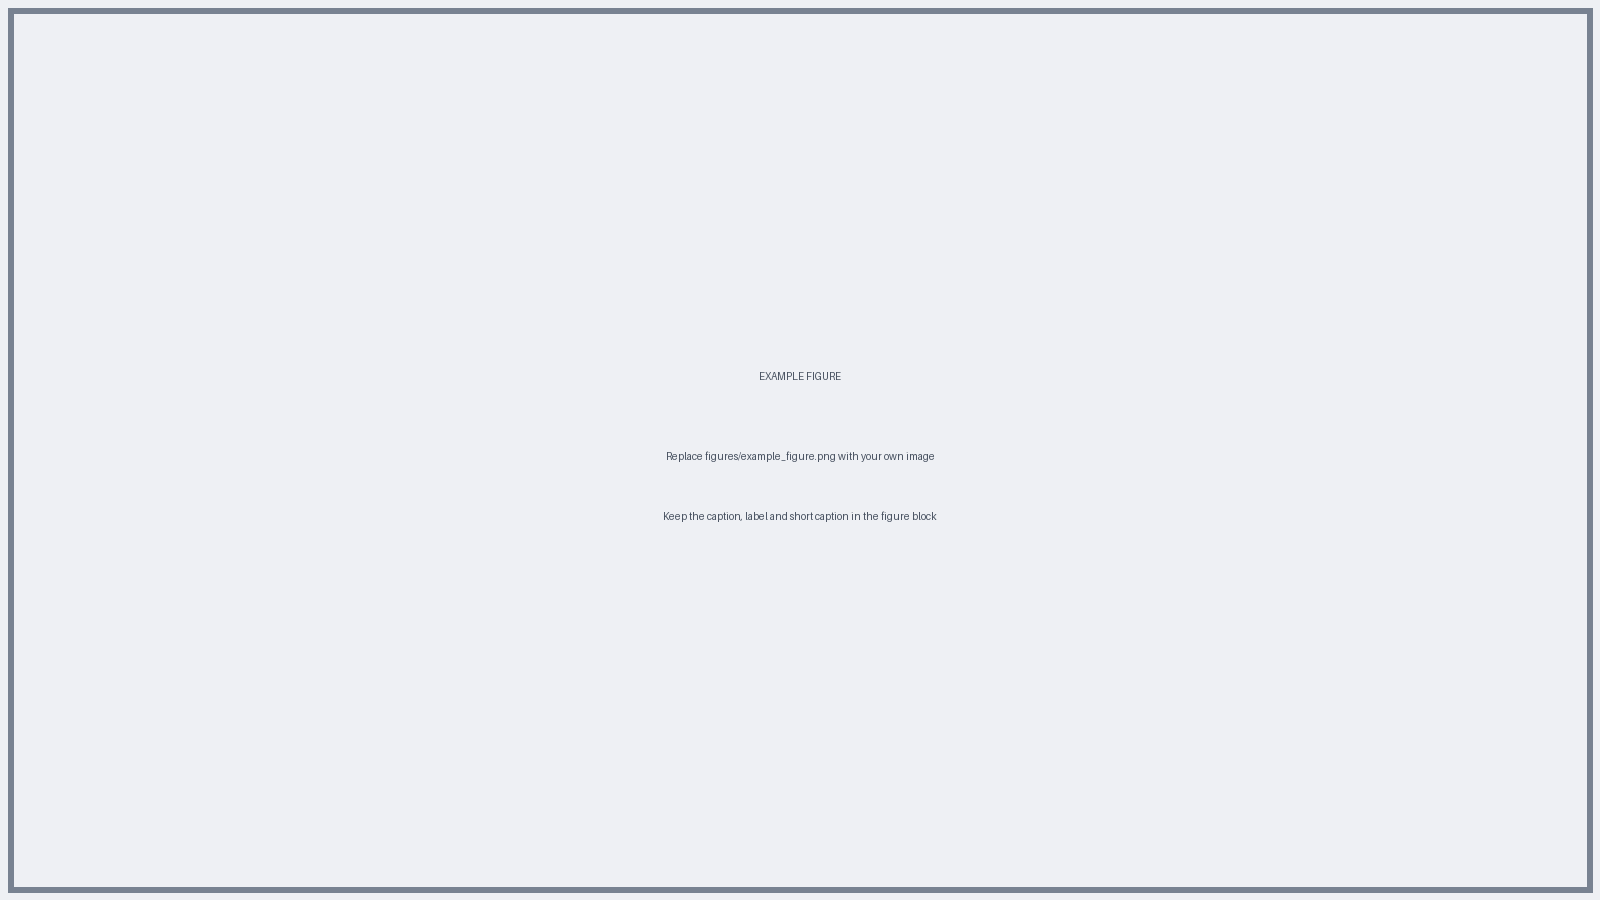
\includegraphics[width=0.85\textwidth]{figures/example_figure.png}
  \caption[Conceptual framework]{Conceptual framework linking [inputs], [evidence layers] and [the study outcome]. Source: author.}
  \label{fig:1.1}
\end{figure}

{[}Paragraph explaining the framework.]

\section{Research Scope}\label{sec:1.7}
\guidance{State what the study covers, where and when, and then state plainly what it does not cover. A clear boundary here prevents scope drift in Chapter 3 and protects you at the defence.}

{[}Scope: materials, sites, period, methods.]

{[}Boundary: this study will not \ldots]

% ====================================================================
%  CHAPTER 2: LITERATURE REVIEW
%  Two levels of subheading are usually enough. Each section should end
%  with what remains unresolved, so that the knowledge gaps in the final
%  section follow from the review rather than being asserted.
% ====================================================================
\chapter{LITERATURE REVIEW}\label{ch:2}

\section{[The Subject and Its Importance]}\label{sec:2.1}

\subsection{[Global and Regional Context]}\label{sec:2.1.1}
{[}Synthesise, do not list. Group studies by what they establish, and say where they disagree \parencite{example_2020_article, example_2021_chapter}.]

\subsection{[Local Context]}\label{sec:2.1.2}
{[}Evidence specific to your country, crop, system or population.]

\section{[The Constraint Your Study Addresses]}\label{sec:2.2}

\subsection{[First Dimension of the Constraint]}\label{sec:2.2.1}
{[}Text.]

\subsection{[Second Dimension of the Constraint]}\label{sec:2.2.2}
{[}Text.]

\section{[Approaches That Have Been Tried]}\label{sec:2.3}
\guidance{Assess each approach on its own terms: what it achieved, under what conditions, and why it has not resolved the problem. Distinguish evidence from extrapolation.}

{[}Text, with a comparative table if it helps. See Table~\ref{tab:2.1}.]

\begin{table}[htbp]
  \centering
  \caption{[Comparison of approaches reported in the literature].}
  \label{tab:2.1}
  \footnotesize
  \begin{tabularx}{\textwidth}{@{}p{0.22\textwidth} p{0.20\textwidth} X@{}}
    \toprule
    \textbf{Approach} & \textbf{Reported outcome} & \textbf{Limitation} \\
    \midrule
    {[}Approach 1] & {[}Outcome] & {[}Limitation] \\
    {[}Approach 2] & {[}Outcome] & {[}Limitation] \\
    \bottomrule
  \end{tabularx}
\end{table}

\section{Methodological Basis for the Study}\label{sec:2.4}
\guidance{Justify the methods you will use in Chapter 3 against alternatives. This is where you show that the design is considered rather than conventional.}

{[}Text.]

\section{Knowledge Gaps Addressed by the Study}\label{sec:2.5}
\guidance{State each gap as a numbered or clearly separated claim, and make sure each one maps onto a specific objective. Close with what the study will not answer.}

{[}First gap.] [Second gap.] [Third gap.]

{[}The study addresses these gaps. It will not answer \ldots]

% ====================================================================
%  CHAPTER 3: MATERIALS AND METHODS
%  Write in the future tense for a proposal. Every objective in Chapter 1
%  needs a method here, and nothing here should exceed the scope set in
%  Section 1.7.
% ====================================================================
\chapter{MATERIALS AND METHODS}\label{ch:3}

\section{Research Design}\label{sec:3.1}
\guidance{Name the design, then say how the objectives map onto its stages and what gates progression from one stage to the next.}

{[}Design and analytical sequence.]

\subsection{Overall Workflow}\label{sec:3.1.1}
The work will proceed through the stages shown in Figure~\ref{fig:3.1}.

\begin{figure}[htbp]
  \centering
  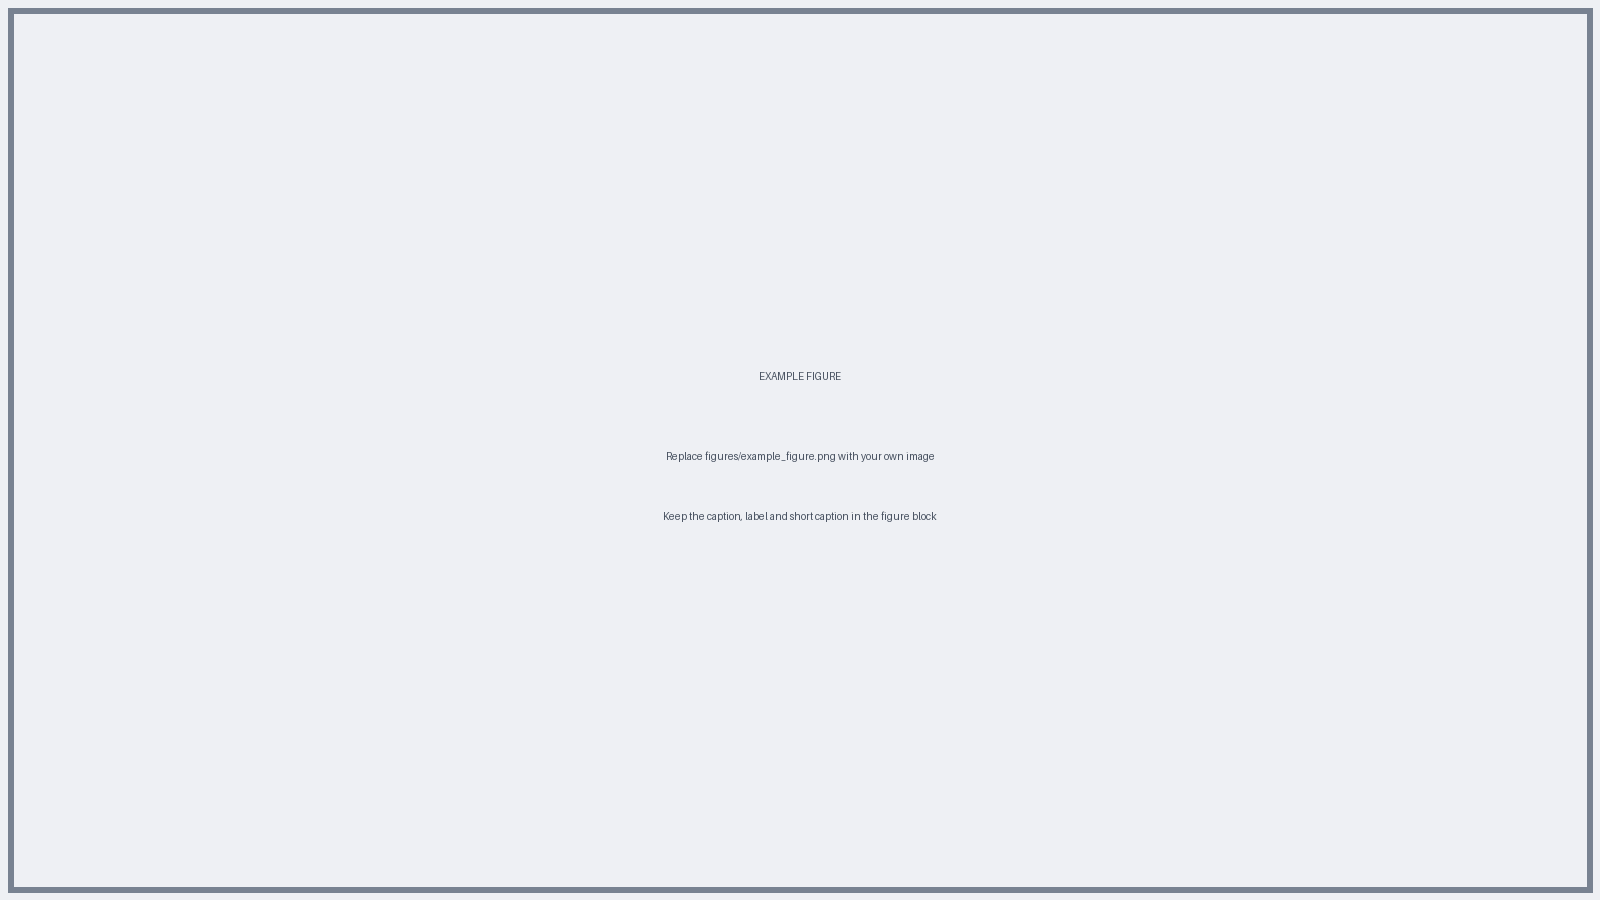
\includegraphics[width=\textwidth]{figures/example_figure.png}
  \caption[Overall study workflow]{Overall study workflow from [first stage] to [final stage]. Source: author.}
  \label{fig:3.1}
\end{figure}

\subsection{Materials, Software and Reproducibility}\label{sec:3.1.2}
\guidance{Record versions. A proposal that names software without versions cannot be reproduced, and examiners notice.}

Table~\ref{tab:3.1} lists the tools to be used.

\begin{table}[htbp]
  \centering
  \caption{Core software, versions and analytical functions.}
  \label{tab:3.1}
  \footnotesize
  \begin{tabularx}{\textwidth}{@{}>{\bfseries}p{0.19\textwidth} X p{0.30\textwidth}@{}}
    \toprule
    Analysis stage & \textbf{Software / version} & \textbf{Primary function} \\
    \midrule
    {[}Stage] & {[}Tool x.y.z] & {[}What it does here] \\
    {[}Stage] & {[}Tool x.y.z] & {[}What it does here] \\
    \bottomrule
  \end{tabularx}
\end{table}

\section{Study Location}\label{sec:3.2}
{[}Where the work will be done, and what facilities that site provides.]

\section{Study Material and Sampling}\label{sec:3.3}

\subsection{Study Material}\label{sec:3.3.1}
{[}Genotypes, accessions, isolates, participants or datasets, with their source and identifiers.]

\subsection{Sampling and Replication}\label{sec:3.3.2}
\guidance{State the experimental unit, the number of independent biological replicates, and what pooling does and does not achieve. Distinguish technical from biological replication.}

{[}Sampling plan, replication and the resulting sample size.]

\subsection{Contingency}\label{sec:3.3.3}
{[}What happens if the material or condition you depend on is not available in time, and the date by which that decision will be taken.]

\section{[Objective 1 Methods]}\label{sec:3.4}
\guidance{One section per objective, with subsections for each procedure. Give thresholds, parameters and acceptance criteria, not just tool names.}

\subsection{[Procedure]}\label{sec:3.4.1}
{[}Method, with parameters, for example an E-value threshold of $1\times10^{-5}$ and coverage of $\geq$~50\%.]

\subsection{[Procedure]}\label{sec:3.4.2}
{[}Method.]

\section{[Objective 2 Methods]}\label{sec:3.5}

\subsection{[Procedure]}\label{sec:3.5.1}
{[}Method.]

\subsection{[Procedure]}\label{sec:3.5.2}
{[}Method.]

\section{Statistical Analysis}\label{sec:3.6}
\guidance{Name the model, the experimental unit, the error control and the reporting convention. Say in advance how assumption failures will be handled, so that the choice is not made after seeing the data.}

{[}Analysis plan, for example: significance at $q<0.05$ after Benjamini-Hochberg correction, with effect sizes and confidence intervals reported alongside adjusted $P$ values.]

\section{Quality Assurance and Quality Control}\label{sec:3.7}
{[}Controls, calibration, exclusion rules, logs and audit trail.]

\section{Ethical and Biosafety Considerations}\label{sec:3.8}
{[}Approvals needed, permissions obtained, waste handling, and a statement of any approvals that fall outside this study.]

\section{Study Limitations and Mitigation}\label{sec:3.9}
Table~\ref{tab:3.2} sets out the anticipated limitations.

\begin{table}[htbp]
  \centering
  \caption{Anticipated limitations, their effects and planned mitigation.}
  \label{tab:3.2}
  \footnotesize
  \begin{tabularx}{\textwidth}{@{}p{0.24\textwidth} p{0.24\textwidth} X@{}}
    \toprule
    \textbf{Limitation} & \textbf{Potential effect} & \textbf{Mitigation} \\
    \midrule
    {[}Limitation] & {[}Effect] & {[}Mitigation] \\
    {[}Limitation] & {[}Effect] & {[}Mitigation] \\
    \bottomrule
  \end{tabularx}
\end{table}

\section{Expected Outputs}\label{sec:3.10}
{[}Datasets, protocols, code, and a statement of what is not an expected output.]

\section{Data Management and Dissemination}\label{sec:3.11}
{[}Storage, backup, identifiers, version control, and how results will be disseminated.]


% ---------------------------- References -----------------------------
\clearpage
\phantomsection
\addcontentsline{toc}{chapter}{REFERENCES}
\printbibliography[title={REFERENCES}]

% ---------------------------- Appendices -----------------------------
% =====================================================================
%  Appendix I -- Budget (landscape)
%  Appendix tables are numbered I.1, I.2, ... and II.1, II.2, ...
% =====================================================================
\clearpage
% Appendices are paginated I, II, III, ... at the bottom centre of the
% landscape page (see \lscapefolio in preamble.tex).
\pagenumbering{Roman}
\pagestyle{empty}
\lscapefolio
\newgeometry{top=2cm,bottom=2cm,left=2cm,right=2cm}
\begin{landscape}
\chapter*{APPENDIX I:}\thispagestyle{empty}\vspace*{-12pt}
\addcontentsline{toc}{chapter}{APPENDIX I: RESEARCH BUDGET}
\renewcommand{\thetable}{I.\arabic{table}}
\setcounter{table}{0}
\begin{center}
  \captionsetup{type=table}
  \caption{Provisional Research Budget}
  \label{tab:A1.1}
  \footnotesize
  \setlength{\tabcolsep}{5pt}\renewcommand{\arraystretch}{1.0}\singlespacing
  \begin{tabularx}{\linewidth}{@{}l Y c c r r@{}}
    \toprule
    \textbf{No.} & \textbf{BUDGET ITEM} & \textbf{UNIT} & \textbf{QTY.} & \textbf{UNIT COST (US\$)} & \textbf{TOTAL (US\$)} \\
    \midrule
    \rowcolor{gray!12}\multicolumn{6}{@{}l}{\textbf{A. [First category]}} \\
    \textbf{1} & {[}Item] & Lot & 1 & 200 & \textbf{200} \\
    \textbf{2} & {[}Item] & Lot & 1 & 150 & \textbf{150} \\
    \multicolumn{5}{r}{\textbf{Subtotal A}} & \textbf{350} \\
    \rowcolor{gray!12}\multicolumn{6}{@{}l}{\textbf{B. [Second category]}} \\
    \textbf{3} & {[}Item] & Pair & 10 & 30 & \textbf{300} \\
    \multicolumn{5}{r}{\textbf{Subtotal B}} & \textbf{300} \\
    \rowcolor{gray!12}\multicolumn{6}{@{}l}{\textbf{C. Contingency}} \\
    \textbf{4} & {[}Repeat assays, price variation, replacement consumables] & Lot & 1 & 120 & \textbf{120} \\
    \multicolumn{5}{r}{\textbf{Subtotal C}} & \textbf{120} \\
    \midrule
    \multicolumn{5}{r}{\textbf{\color{red}GRAND TOTAL}} & \textbf{\color{red}US\$770} \\
    \bottomrule
  \end{tabularx}
\end{center}
\end{landscape}
\restoregeometry

% =====================================================================
%  Appendix II -- Work plan (landscape)
%  \ding{108} filled circle = main activity, \ding{109} open circle =
%  partial activity. The legend below the table explains both.
% =====================================================================
\clearpage
\newgeometry{top=2cm,bottom=2cm,left=2cm,right=2cm}
\begin{landscape}
\chapter*{APPENDIX II:}\thispagestyle{empty}
\addcontentsline{toc}{chapter}{APPENDIX II: PROJECT WORK PLAN}
\renewcommand{\thetable}{II.\arabic{table}}
\setcounter{table}{0}
\definecolor{m1}{RGB}{222,235,247}
\definecolor{m2}{RGB}{198,225,245}
\definecolor{m3}{RGB}{170,207,237}
\definecolor{m4}{RGB}{146,203,236}
\definecolor{m5}{RGB}{160,220,245}
{\footnotesize\singlespacing\renewcommand{\arraystretch}{1.0}
\setlength{\tabcolsep}{4pt}
\begin{longtable}{@{}l p{7.2cm} >{\columncolor{m1}\centering\arraybackslash}p{1.35cm} >{\columncolor{m2}\centering\arraybackslash}p{1.35cm} >{\columncolor{m3}\centering\arraybackslash}p{1.35cm} >{\columncolor{m4}\centering\arraybackslash}p{1.35cm} >{\columncolor{m5}\centering\arraybackslash}p{1.35cm} p{5.6cm}@{}}
  \caption{Project Work Plan}\label{tab:A2.1}\\
  \toprule
  \rowcolor{gray!20}\textbf{No.} & \textbf{Activity} & \textbf{Month 1} & \textbf{Month 2} & \textbf{Month 3} & \textbf{Month 4} & \textbf{Month 5} & \textbf{Expected Output/Milestone} \\
  \midrule
  \endfirsthead
  \toprule
  \rowcolor{gray!20}\textbf{No.} & \textbf{Activity} & \textbf{Month 1} & \textbf{Month 2} & \textbf{Month 3} & \textbf{Month 4} & \textbf{Month 5} & \textbf{Expected Output/Milestone} \\
  \midrule
  \endhead
  \bottomrule
  \endlastfoot
  \textbf{1} & {[}Proposal refinement and approvals] & \ding{108} & & & & & {[}Approved protocol] \\ \midrule
  \textbf{2} & {[}Set up materials, environment or field site] & \ding{108} & \ding{109} & & & & {[}Ready to begin] \\ \midrule
  \textbf{3} & {[}Data generation] & & \ding{108} & \ding{108} & \ding{109} & & {[}Dataset] \\ \midrule
  \textbf{4} & {[}Analysis] & & & \ding{109} & \ding{108} & \ding{108} & {[}Results] \\ \midrule
  \textbf{5} & {[}Writing and dissemination] & & & & \ding{109} & \ding{108} & {[}Draft dissertation] \\
\end{longtable}
\vspace{-6pt}\noindent\ding{108}\,= main period of activity;\quad \ding{109}\,= partial, preparatory or follow-up activity.
}
\end{landscape}
\restoregeometry
\stoplscapefolio


\end{document}
